\chapter{La gravitación}\label{ch:g9:gravitation}

Una manzana se suelta de su \omterm{def:g5:series-parallel-circuits:parallel}{rama} y cae. La \omterm{def:g2:moon-in-the-sky:moon}{Luna}, encima del
mismo huerto, no. Durante miles de años estos parecieron dos hechos sin
relación --- hasta que una intuición genial los unió: la
\omterm{def:g2:moon-in-the-sky:moon}{Luna} \emph{está} cayendo, sin parar, alrededor de la Tierra,
sostenida por el mismísimo tirón que reclama a la manzana. Una sola ley
para el huerto y para el cielo --- la ecuación más atrevida que se
había escrito hasta aquel día, y con ella se abre tu último año de este
libro.

\section{La atracción universal}

\begin{definition}[Gravitación]\label{def:g9:gravitation:gravitation}
La \emph{gravitación}\index{gravitación} es la atracción mutua entre
todas las \omterm{def:g3:measuring-mass:mass}{masas}: cada porción de materia del universo tira de todas las
demás. Es la \omterm{def:g2:pushes-and-pulls:force}{fuerza} sin contacto que conociste hace años como ``el
tirón de la Tierra'' --- revelada ahora como universal: la Tierra tira
de la manzana, la manzana tira de la Tierra, la \omterm{def:g2:moon-in-the-sky:moon}{Luna} tira de los
mares, el Sol tira de los \omterm{def:g4:solar-system:planet}{planetas} y dos libros de un estante tiran
el uno del otro, debilísimamente, para siempre.
\end{definition}

\begin{proposition}[La ley de la gravitación universal]\label{prop:g9:gravitation:law}
Dos cuerpos de \omterm{def:g3:measuring-mass:mass}{masas} $m_A$ y $m_B$ (en \unit{kg}), con sus centros a
una distancia $d$ (en \unit{m}), se atraen con
\omterm{def:g2:pushes-and-pulls:force}{fuerzas} iguales y opuestas a lo largo de la recta que los une, de
valor
\[
F = G \times \frac{m_A \times m_B}{d^2},
\]
con $F$ en newtons (\unit{N}) --- la \omterm{def:g6:measurement-in-science:measuring}{unidad} de
\omterm{def:g2:pushes-and-pulls:force}{fuerza} cuya historia completa empieza en el capítulo siguiente
--- y con $G = \qty{6.67e-11}{N.m^2/kg^2}$, la \emph{constante de
\omterm{def:g9:gravitation:gravitation}{gravitación}}, el mismo número en todo el universo. La
\omterm{def:g2:pushes-and-pulls:force}{fuerza} crece con cada \omterm{def:g3:measuring-mass:mass}{masa} y muere con el
\emph{cuadrado} de la distancia: al doble de lejos, cuatro veces más
débil; a diez veces la distancia, cien veces más débil.
\end{proposition}

\begin{omfigure}
\begin{tikzpicture}[scale=0.85]
  \draw[thick, fill=omDef, fill opacity=0.4] (1.4,1.4) circle (0.65);
  \node[font=\small] at (1.4,1.4) {$m_A$};
  \draw[thick, fill=omThm, fill opacity=0.4] (8.6,1.4) circle (0.45);
  \node[font=\small] at (8.6,1.4) {$m_B$};
  \draw[-Stealth, very thick, omThm] (2.15,1.4) -- (3.55,1.4);
  \draw[-Stealth, very thick, omDef] (8.05,1.4) -- (6.65,1.4);
  \draw[Stealth-Stealth, omExo] (1.4,0.45) -- (8.6,0.45);
  \node[below, font=\small, omExo] at (5.0,0.35) {$d$};
  \node[above, font=\small] at (5.0,1.75)
    {tirones iguales, sentidos opuestos --- siempre los dos};
\end{tikzpicture}

{\small La \omterm{def:g9:gravitation:gravitation}{gravitación} universal: dos \omterm{def:g3:measuring-mass:mass}{masas}, dos tirones iguales y
opuestos a lo largo de la recta que las une --- la manzana tira de la
Tierra exactamente con la misma \omterm{def:g2:pushes-and-pulls:force}{fuerza} con que la Tierra tira de la
manzana.}
\end{omfigure}

\begin{example}[Leer la ley]\label{ex:g9:gravitation:reading}
Todos los rasgos de la fórmula hablan. Las \omterm{def:g3:measuring-mass:mass}{masas} se multiplican: dobla
cualquiera de las dos compañeras y doblarás la \omterm{def:g2:pushes-and-pulls:force}{fuerza}. La distancia
va al cuadrado en el denominador: la gravedad es un susurro que se
apaga a toda prisa --- la dilución del inverso del cuadrado que
volverás a encontrarte con la \omterm{def:g1:light-and-shadows:source}{luz} y con el \omterm{def:g3:sound-around-us:sound}{sonido}, pues es
la geometría de todo lo que se reparte por el espacio. Y el tamaño
minúsculo de $G$ --- once ceros antes de su primera cifra --- proclama a la
\omterm{def:g9:gravitation:gravitation}{gravitación} la enclenque de las \omterm{def:g2:pushes-and-pulls:force}{fuerzas} de la
naturaleza: gobierna el cosmos solo porque las \omterm{def:g3:measuring-mass:mass}{masas} de ahí arriba son
monstruosas y nada la cancela.
\end{example}

\begin{example}[Por qué los estantes no se aplastan]\label{ex:g9:gravitation:books}
Dos libros de \qty{1}{kg}, con los centros a \qty{0.1}{m}:
\[
F = \num{6.67e-11} \times \frac{1 \times 1}{0.1^2}
= \qty{6.67e-9}{N}
\]
--- unas milmillonésimas de newton, el \omterm{def:g4:weight-and-mass:weight}{peso} de la mota de polvo de
una mota de polvo. Ahora la Tierra y la manzana: sustituye uno de los
libros por \qty{5.97e24}{kg} de \omterm{def:g4:solar-system:planet}{planeta} y la distancia por su radio
de \qty{6.4e6}{m}, y esa misma ley entrega el tirón familiar de una
tarde en el huerto. Universal significa universal --- solo las \omterm{def:g3:measuring-mass:mass}{masas}
deciden quién se entera.
\end{example}

\section{La Luna que cae}

\begin{example}[El cañón de la montaña]\label{ex:g9:gravitation:cannon}
El experimento mental de la propia intuición. Dispara horizontalmente
una bala de cañón desde una cima alta: describe un arco y aterriza.
Dispárala más rápido: aterriza más lejos --- con el tirón de la Tierra
doblándole el camino todo el rato. Ahora imagina dispararla tan rápido
que, mientras cae, la superficie de la Tierra redonda \emph{se curve
alejándose por debajo al mismo ritmo}: la bala cae sin parar y no
aterriza nunca --- da vueltas al \omterm{def:g4:solar-system:planet}{planeta}. Esa caída perpetua tiene
un nombre conocido: una \emph{\omterm{def:g6:sun-earth-moon:axisorbit}{órbita}}. Nada sujeta ``arriba'' a un
cuerpo en \omterm{def:g6:sun-earth-moon:axisorbit}{órbita}; está cayendo con estilo.
\end{example}

\begin{omfigure}
\begin{tikzpicture}[scale=0.85]
  % the curving Earth: only the upper limb of a much larger circle
  \fill[omDef, opacity=0.25] (-1.01,0.23) arc (106:74:20)
    -- (10.01,-0.9) -- (-1.01,-0.9) -- cycle;
  \draw[thick] (-1.01,0.23) arc (106:74:20);
  % the mountain and its gun
  \draw[thick, fill=omExo!30]
    (-1.1,0.2) -- (0.25,2.3) -- (1.3,0.72) -- cycle;
  \draw[thick, fill=omExo!60] (0.0,2.18) rectangle (0.55,2.42);
  \node[left, font=\small] at (-0.85,2.3) {el cañón de la montaña};
  % three shots, each faster than the last
  \draw[omThm, thick] (0.55,2.32)
    .. controls (1.6,2.25) .. (2.4,0.9);
  \draw[omThm, thick] (0.55,2.35)
    .. controls (2.8,2.25) .. (4.9,1.0);
  \draw[omThm, thick] (0.55,2.38)
    .. controls (4.2,2.35) .. (7.5,0.8);
  \node[right, font=\small, omThm] at (1.9,3.0)
    {más rápido: más lejos};
  % fast enough: the fall closes into an orbit
  \draw[omMeth, very thick, dashed] (0.3,2.35) arc (101:73:21.76);
  \node[right, font=\small, omMeth] at (6.4,3.35)
    {bastante rápido: la caída se hace órbita};
\end{tikzpicture}

{\small El cañón de la montaña: cada disparo más rápido cae más lejos
alrededor de la Tierra curvada --- hasta que la caída y la curvatura
coinciden y la bala orbita.}
\end{omfigure}

\begin{proposition}[Lo que gobierna la gravitación]\label{prop:g9:gravitation:runs}
Una ley, el cielo entero: la \omterm{def:g2:moon-in-the-sky:moon}{Luna} es la bala de cañón eterna de
la Tierra, cayendo a nuestro alrededor una vez al mes; los
\omterm{def:g4:solar-system:planet}{planetas} caen igual alrededor del Sol --- los más cercanos más
deprisa, como exige el inverso del cuadrado; los cometas se lanzan
desde la oscuridad en largos bucles de caída; y todos los satélites
artificiales --- ojos meteorológicos, balizas de navegación, la
estación tripulada que da una vuelta cada noventa minutos --- montan en
las matemáticas del cañón de la montaña. Nada está suspendido en los
cielos. Todo cae, y falla el blanco.
\end{proposition}

\begin{example}[Las mareas: la Luna tira de vuelta]\label{ex:g9:gravitation:tides}
La mutualidad tiene una firma escrita en el agua. El tirón de la
\omterm{def:g2:moon-in-the-sky:moon}{Luna} sobre la Tierra es más fuerte en el océano que la mira y más
débil en el lado opuesto --- así que los mares se amontonan suavemente
hacia la \omterm{def:g2:moon-in-the-sky:moon}{Luna} y en dirección contraria a la vez, y, mientras la
Tierra gira por debajo de los montones, las costas ven subir y bajar el
agua: las \emph{mareas}, dos veces casi todos los días. El Sol echa una
mano --- alineado en luna nueva y en \omterm{ex:g2:moon-in-the-sky:shapes}{luna llena} para las grandes
mareas vivas. Los pescadores llevan milenios leyendo la
\omterm{def:g2:moon-in-the-sky:moon}{Luna}; la ley se la lee a ella.
\end{example}

\begin{remark}[Lo que la ley no dice]\label{rem:g9:gravitation:notsay}
La gran ecuación calcula la \omterm{def:g2:pushes-and-pulls:force}{fuerza} con una exquisita exactitud y
no explica ni una pizca de \emph{cómo} se agarran dos cuerpos a través
de la nada vacía --- su propio autor declaró la pregunta abierta y la
dejó, magníficamente, sin responder. Existen respuestas más profundas
--- los años de universidad de este curso alcanzan la moderna, en la
que la \omterm{def:g3:measuring-mass:mass}{masa} curva la mismísima geometría que habita ---, pero
todos los físicos honrados desde entonces han repetido la lección que
puedes llevarte de esta página: una ley puede ser perfectamente útil,
perfectamente comprobada y guardar aún su secreto último.
\end{remark}

\begin{omfigure}
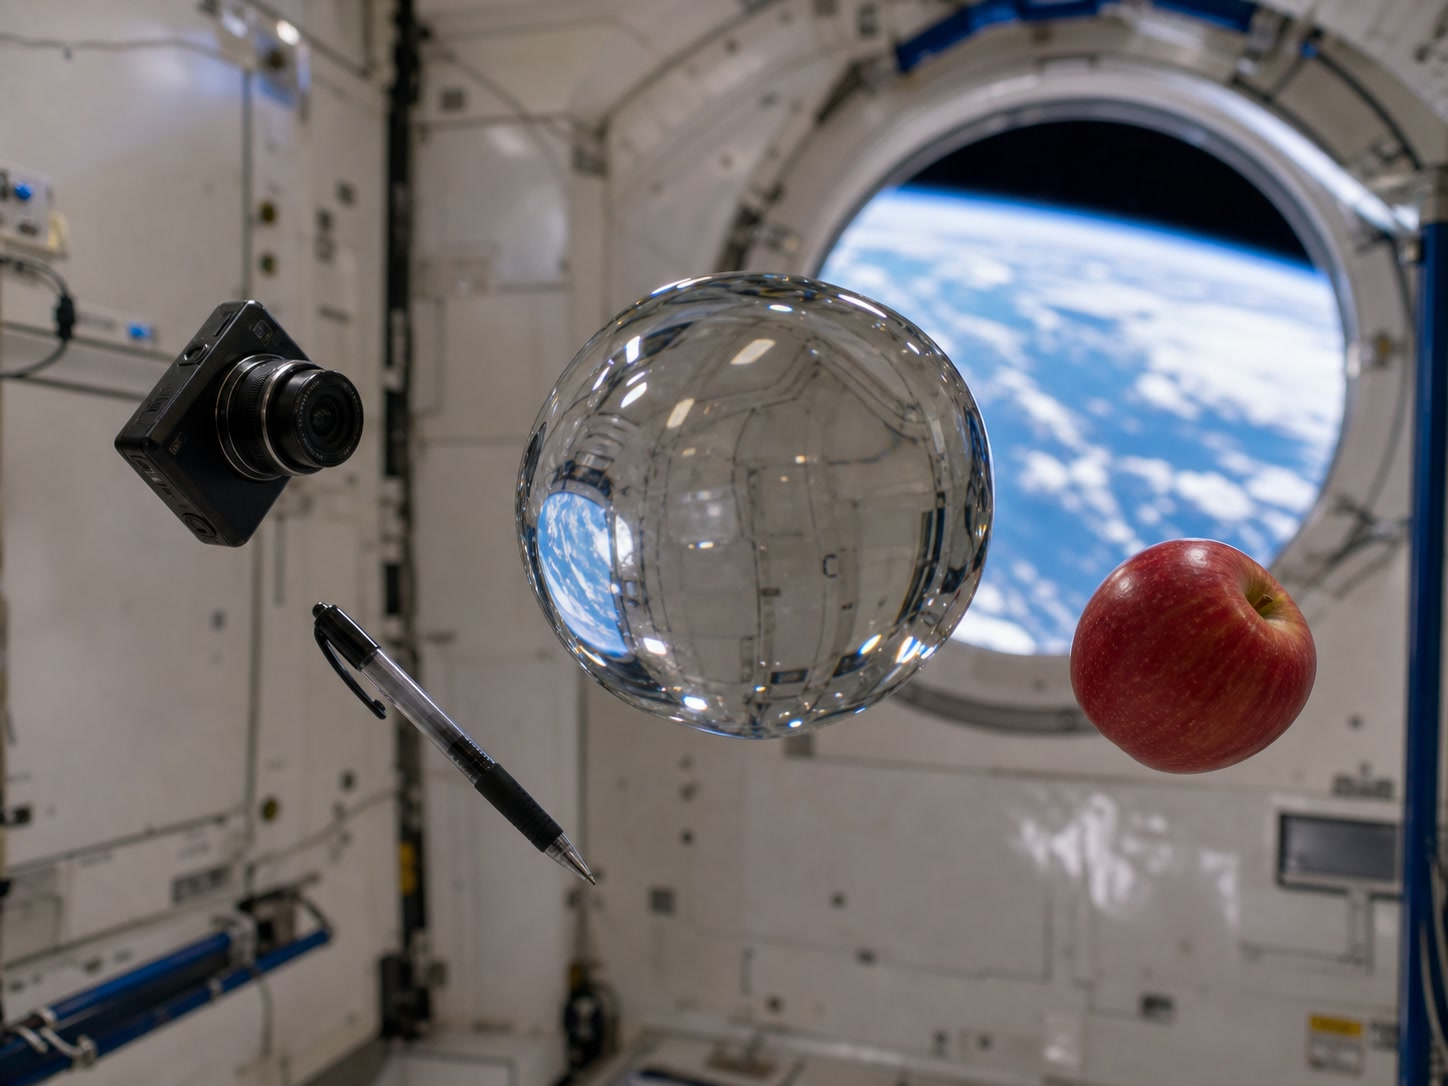
\includegraphics[width=0.5\linewidth]{images/book1/ai/g9-gravitation-weightless.jpg}

{\small La caída libre, vivida a diario: la estación espacial y todo lo que hay dentro caen juntos alrededor de la Tierra, así que nada aprieta contra nada --- las cámaras, los bolígrafos, las manzanas y el agua flotan.}
\end{omfigure}

\section{Ejercicios}

\begin{exercise}[$\star$]\label{exo:g9:gravitation:1}
Enuncia la ley de la \omterm{def:g9:gravitation:gravitation}{gravitación} universal --- fórmula,
\omterm{def:g6:measurement-in-science:measuring}{unidades} y los dos rasgos (\omterm{def:g3:measuring-mass:mass}{masas} y distancia) con palabras.
\end{exercise}

\begin{exercise}[$\star$]\label{exo:g9:gravitation:2}
La Tierra tira de la manzana con \qty{1}{N}. ¿Con qué
\omterm{def:g2:pushes-and-pulls:force}{fuerza} tira la manzana de la Tierra? ¿Por qué solo uno de los dos
acelera de forma visible?
\end{exercise}

\begin{exercise}[$\star$]\label{exo:g9:gravitation:3}
Dos satélites orbitan a distancias $d$ y $2d$ del centro de la
Tierra. Compara las \omterm{def:g2:pushes-and-pulls:force}{fuerzas} gravitatorias sobre ellos (con \omterm{def:g3:measuring-mass:mass}{masas}
iguales). ¿Y a $10 d$?
\end{exercise}

\begin{exercise}[$\star$]\label{exo:g9:gravitation:4}
Calcula la atracción entre dos bailarines de \qty{80}{kg} separados
\qty{0.5}{m} --- y comenta el romance frente a la
\omterm{def:g9:gravitation:gravitation}{gravitación}.
\end{exercise}

\begin{exercise}[$\star$]\label{exo:g9:gravitation:5}
En la historia del cañón de la montaña, ¿qué dos ritmos coinciden
exactamente para el disparo que orbita? ¿Qué es una
\omterm{def:g6:sun-earth-moon:axisorbit}{órbita}, en tres palabras?
\end{exercise}

\begin{exercise}[$\star$]\label{exo:g9:gravitation:6}
``Los astronautas flotan porque ahí arriba no hay gravedad''.
Demuele esto con la bala de cañón: ¿qué están haciendo la estación y la
tripulación?
\end{exercise}

\begin{exercise}[$\star$]\label{exo:g9:gravitation:7}
¿Por qué gobierna el cosmos la \omterm{def:g9:gravitation:gravitation}{gravitación}, la enclenque de la
naturaleza? Dos razones del capítulo.
\end{exercise}

\begin{exercise}[$\star$]\label{exo:g9:gravitation:8}
¿De dónde vienen las mareas y por qué hay dos casi todos los días?
¿Cuándo llegan las más grandes?
\end{exercise}

\begin{exercise}[$\star\star$]\label{exo:g9:gravitation:9}
La \omterm{def:g2:moon-in-the-sky:moon}{Luna} (\qty{7.3e22}{kg}) orbita a \qty{3.8e8}{m} de la
Tierra (\qty{5.97e24}{kg}). Calcula su atracción, en notación
científica de principio a fin --- y admira cuántas cifras lleva la
potencia de diez de la respuesta.
\end{exercise}

\begin{exercise}[$\star\star$]\label{exo:g9:gravitation:10}
En la superficie de la \omterm{def:g2:moon-in-the-sky:moon}{Luna}, tu \omterm{def:g4:weight-and-mass:weight}{peso} encogía hasta una
sexta parte (acuérdate de los astronautas dando saltitos). Con los dos
mandos de la ley --- la \omterm{def:g3:measuring-mass:mass}{masa} menor de la \omterm{def:g2:moon-in-the-sky:moon}{Luna} y su radio
menor ---, explica cómo puede salir una sexta parte de un cuerpo ochenta
veces más ligero que la Tierra.
\end{exercise}

\begin{exercise}[$\star\star$]\label{exo:g9:gravitation:11}
Mercurio le da la vuelta al Sol en $88$ días; Neptuno, en $165$ años.
Lee esta pauta a partir del inverso del cuadrado: ¿qué le hace al
agarre del Sol el que la gravedad se apague con la distancia, y qué le
hace por tanto al ritmo de la familia exterior?
\end{exercise}

\begin{exercise}[$\star\star\star$]\label{exo:g9:gravitation:12}
Un satélite geoestacionario cuelga aparentemente inmóvil sobre un punto
del ecuador --- las antenas parabólicas no se mueven nunca. Concilia la
apariencia con la \cref{prop:g9:gravitation:runs}: ¿cuál tiene que ser
su periodo orbital, en qué sentido tiene que dar vueltas y por qué
``colgar'' significa aquí ``caer en perfecta sincronía con la Tierra que
gira''?
\end{exercise}

\section{Problema: la herencia de la bala de cañón}

\begin{problem}[{Problema de fin de semana --- del huerto a la órbita;
la manzana, el cañón y la Luna auditados con una sola ley; el tablero
de lanzamiento de satélites}]\label{pb:g9:gravitation:1}
Una tarde en la mesa de divulgación de la agencia espacial: una sola
ley, $G = \qty{6.67e-11}{N.m^2/kg^2}$, \omterm{def:g3:measuring-mass:mass}{masa} de la Tierra
\qty{5.97e24}{kg} y radio de la Tierra \qty{6.4e6}{m}.

\medskip\noindent\textbf{Parte I --- La auditoría de la manzana.}
\begin{enumerate}
  \item Calcula el tirón de la Tierra sobre una manzana de
        \qty{0.1}{kg} en la superficie (con los centros separados un
        radio terrestre).
  \item ¿Con qué \omterm{def:g2:pushes-and-pulls:force}{fuerza} tira la manzana de la Tierra? Di la
        palabra que usa la ley para esta contabilidad de doble
        sentido.
  \item Levanta la manzana hasta el doble del radio terrestre desde
        el centro. ¿Qué le pasa al tirón?
  \item Un visitante pregunta por qué la fórmula usa la distancia al
        \emph{centro} de la Tierra y no al suelo. Ofrécele la
        respuesta corta y honrada (tira el \omterm{def:g4:solar-system:planet}{planeta} entero, y sus
        tirones repartidos suman como si vinieran del centro --- un
        teorema que el gran autor necesitó años para demostrar).
\end{enumerate}

\medskip\noindent\textbf{Parte II --- El tablero de lanzamiento.}
\begin{enumerate}[resume]
  \item El satélite de hoy tiene una \omterm{def:g3:measuring-mass:mass}{masa} de \qty{2000}{kg}. ¿Su
        \omterm{def:g4:weight-and-mass:weight}{peso} en la superficie, según la ley? (O según el atajo
        que nombra el capítulo siguiente: unos \qty{9.8}{N} por
        \omterm{def:g3:measuring-mass:units}{kilogramo}.)
  \item En su \omterm{def:g6:sun-earth-moon:axisorbit}{órbita} de trabajo a \qty{1.28e7}{m} del centro
        --- dos radios terrestres ---, ¿qué fracción de su
        \omterm{def:g4:weight-and-mass:weight}{peso} en la superficie sigue ejerciendo sobre él la
        gravedad?
  \item ``¿Entonces ahí arriba sigue habiendo gravedad de verdad?''.
        Confírmalo con el número --- y explica qué está haciendo el
        satélite con ese tirón en lugar de estrellarse.
  \item El comentario del lanzamiento dice que ``la
        \omterm{def:g7:motion-average-speed:formula}{velocidad} orbital tiene que igualar a la caída''. Vuelve
        a contar en dos frases la historia del cañón de la montaña
        para el folleto de los visitantes.
\end{enumerate}

\medskip\noindent\textbf{Parte III --- El libro de cuentas de la
\omterm{def:g2:moon-in-the-sky:moon}{Luna}.}
\begin{enumerate}[resume]
  \item Con la \omterm{def:g2:moon-in-the-sky:moon}{Luna} a \qty{3.8e8}{m}, ¿a cuántos radios
        terrestres viaja? (Un decimal.)
  \item Por el inverso del cuadrado, ¿a qué fracción aproximada de
        su \omterm{def:g2:pushes-and-pulls:force}{fuerza} en la superficie se ha apagado allí la gravedad?
        (Eleva al cuadrado tu respuesta anterior.)
  \item La gran intuición, vuelta a contar: la manzana del huerto
        cae unos cinco \omterm{def:g2:measuring-length:units}{metros} en su primer segundo; la
        \omterm{def:g2:moon-in-the-sky:moon}{Luna}, cada segundo, ``cae'' hacia la Tierra apenas un
        milímetro --- y sin embargo no llega nunca. Conecta los dos
        hechos con tus respuestas 9 y 10: ¿por qué es miles de veces
        más suave la caída de la \omterm{def:g2:moon-in-the-sky:moon}{Luna}, y por qué es sin fin?
  \item Cierra la tarde de divulgación: una ley, tres intérpretes
        --- manzana, satélite y \omterm{def:g2:moon-in-the-sky:moon}{Luna}. Escribe la frase de cierre
        del tablero que los une.
\end{enumerate}
\end{problem}
